%
% Defines for camera-ready version:
%  - Use \ifEurocrypt <bla> \else <wla> \fi throughout paper
%  - Also, can use \ifNotEurocrypt <bla> \fi
%
\newif\ifEurocrypt
%\Eurocrypttrue    % uncomment for camera-ready version
\newif\ifNotEurocrypt
\ifEurocrypt\NotEurocryptfalse\else\NotEurocrypttrue\fi

\ifEurocrypt
\documentclass{llncs}
\pagestyle{plain}
\else
\documentclass[10pt]{extarticle}
\fi

\usepackage{adjustbox}
\usepackage{array}
\usepackage{amsmath}
\usepackage{amssymb}
\usepackage{amsfonts}
\ifNotEurocrypt
    \usepackage{amsthm}
\fi
\usepackage{authblk}    % for \author[1] and \affil[1]
\usepackage{bm}
\usepackage{booktabs}
\usepackage{cite}
%\usepackage{forest}
\ifNotEurocrypt
    \usepackage[margin=1in,bmargin=1in]{geometry} % 1 inch margins
\fi
%\usepackage[acronym,automake,nomain]{glossaries}
%\usepackage{glossaries-extra}
\usepackage{hyperref}
\usepackage{hyphenat}
\usepackage[utf8]{inputenc}
\usepackage{lscape}
%\usepackage{times}         % for theme with Times
\ifNotEurocrypt
    \usepackage{libertine}      % for theme with cooler Biolinum font
\fi
\usepackage{makecell}
\ifNotEurocrypt
    \usepackage{titlesec}
\fi
\usepackage{titling}
\usepackage{transparent}
\usepackage[dvipsnames]{xcolor}
%\usepackage{enumitem}
\usepackage{xspace}
\usepackage[capitalize]{cleveref}

% for some reason, these are not defined in cleveref and I was getting '??' in my crefs to subsubsections in the appendix
\crefformat{subsubsubappendix}{Appendix #2#1#3}
\crefmultiformat{subsubsubappendix}{Appendices #2#1#3}{ and~#2#1#3}{, #2#1#3}{, and~#2#1#3}
%
% Colors
%
\definecolor{myBlueColor}{HTML}{268BD2}
\definecolor{myYellowColor}{HTML}{B58900}
\definecolor{myGreenColor}{HTML}{859900}
\definecolor{myRedColor}{HTML}{DC322F}
\definecolor{mygray}{gray}{0.5}
\newcommand{\myblue}[1]{\textcolor{myBlueColor}{#1}}
\newcommand{\myred}[1]{\textcolor{myRedColor}{#1}}
\newcommand{\red}[1]{\textcolor{red}{#1}}
\newcommand{\myyellow}[1]{\textcolor{myYellowColor}{#1}}
\newcommand{\mygreen}[1]{\textcolor{myGreenColor}{#1}}
\newcommand{\g}[1]{\textcolor{ForestGreen}{#1}}
\newcommand{\m}[1]{\myyellow{#1}}
\newcommand{\N}[1]{\myred{#1}}

%
% Math notation
%
\newcommand{\bezout}{B\'ezout\xspace}
\newcommand{\Gr}{\ensuremath{\mathbb{G}}\xspace}
\newcommand{\Z}{\ensuremath{\mathbb{Z}}\xspace}
\newcommand{\Zp}{\ensuremath{\Z_p}\xspace}
\newcommand{\lagr}{\ensuremath{\mathcal{L}}\xspace}
\newcommand{\Oh}{\ensuremath{\mathcal{O}}}  % for Big-Oh notation
\newcommand{\primes}{\ensuremath{\mathsf{Primes}}\xspace}

\newcommand{\vect}[1]{\ensuremath{\bm{#1}}}
\newcommand{\matr}[1]{\ensuremath{\mathbf{#1}}}
\newcommand{\diag}{\ensuremath{\mathsf{diag}}}
\newcommand{\dft}{\ensuremath{\mathsf{DFT}}}
\newcommand{\invdft}{\ensuremath{\mathsf{DFT}^{-1}}}

% For adding "--- a_i ---" lines to a matrix A whose rows are a_i's
% e.g., \begin{bmatrix} \llongdash a_i \rlongdash\end{bmatrix}
\makeatletter
\newcommand{\longdash}[1][2em]{%
    \makebox[#1]{$\m@th\smash-\mkern-7mu\cleaders\hbox{$\mkern-2mu\smash-\mkern-2mu$}\hfill\mkern-7mu\smash-$}}
\makeatother
\newcommand{\omitskip}{\kern-\arraycolsep}
\newcommand{\llongdash}[1][1.5em]{\longdash[#1]\omitskip}
\newcommand{\rlongdash}[1][1.5em]{\omitskip\longdash[#1]}

%
% Crypto things
%
\newcommand{\poly}{\ensuremath{\mathsf{poly}}\xspace}
\newcommand{\negl}{\ensuremath{\mathsf{negl}}\xspace}
\newcommand{\adv}{\ensuremath{\mathcal{A}}\xspace}
\newcommand{\badv}{\ensuremath{\mathcal{B}}\xspace}

%
% Comments and annotations
%
\newcommand{\authnote}[2]{{\footnotesize\textcolor{red}{{\textbf{#1:} }\textcolor{blue}{#2}}}}
\newcommand{\anote}[1]{{\authnote{Alin}{#1}}}
\newcommand{\atodo}[1]{{\authnote{Alin (\textbf{TODO})}{#1}}}

\newcommand{\nop}{\myred{$\times$}}
\newcommand{\yep}{\textcolor{ForestGreen}{\textbf{\checkmark}}}
\newcommand{\idk}{{?}}

%
% Tables
%
\newcolumntype{R}[2]{%
    >{\adjustbox{angle=#1,lap=\width-(#2)}\bgroup}%
    l%
    <{\egroup}%
}
% e.g. \rot{60}{1em}{Title} rotates the title "Title" by 60 degrees and leaves 1em of space in the column
\newcommand*\rot[2]{\multicolumn{1}{R{#1}{#2}}}% no optional argument here, please!

%
% Formatting
%
\newcommand{\eg}{\textit{e.g.,}\xspace}
\newcommand{\api}{\smallskip \hangindent=\parindent \hangafter=1 \noindent}
\newcommand{\parhead}[1]{\medskip\noindent{\bfseries\boldmath\ignorespaces{#1}}}
\newcommand{\alg}[1]{\ensuremath{\boldmath\mathsf{#1}}}
% for setting custom font sizes
\newlength{\mysize}
\newcommand{\myfontsize}[1]{\setlength{\mysize}{#1pt}%
    \fontsize{\mysize}{1.2\mysize}\selectfont}

% For commenting inside algorithm blocks built using figure/tabular, not algorithmic
\newcommand{\comment}[1]{\ifEurocrypt\scriptsize\else\footnotesize\fi$\triangleright$ \textcolor{mygray}{\textit{#1}}}
\newcommand{\commentcont}[1]{\ifEurocrypt\scriptsize\else\footnotesize\fi\phantom{$\triangleright$} \textcolor{mygray}{\textit{#1}}}

%
% VC things
%

\newcommand{\pp}{\ensuremath{\mathsf{PP}}\xspace}
\newcommand{\prk}{\ensuremath{\mathsf{prk}}\xspace}
\newcommand{\vrk}{\ensuremath{\mathsf{vrk}}\xspace}
\newcommand{\upk}{\ensuremath{\mathsf{upk}}\xspace}

\newcommand{\vcsetup}{\ensuremath{\mathsf{VC.Setup}}\xspace}
\newcommand{\vccommit}{\ensuremath{\mathsf{VC.Commit}}\xspace}
\newcommand{\vcopenpos}{\ensuremath{\mathsf{VC.ProvePos}}\xspace}
\newcommand{\vcverifypos}{\ensuremath{\mathsf{VC.VerifyPos}}\xspace}
\newcommand{\vcverifyupk}{\ensuremath{\mathsf{VC.VerifyUPK}}\xspace}
\newcommand{\vcdigupdate}{\ensuremath{\mathsf{VC.UpdateDig}}\xspace}
\newcommand{\vcproofupdate}{\ensuremath{\mathsf{VC.UpdateProof}}\xspace}
\newcommand{\vcopenall}{\ensuremath{\mathsf{VC.ProveAll}}\xspace}

%
% Theorems, defs, lemmas, etc.
%
\ifNotEurocrypt
\theoremstyle{definition}
\newtheorem{definition}{Definition}[section]
\newtheorem{theorem}{Theorem}[section]
\newtheorem{corollary}{Corollary}[theorem]
\newtheorem{lemma}[theorem]{Lemma}
\fi


\title{\textbf{How to compute all Pointproofs}} %from Hidden-Order Groups}}

\ifNotEurocrypt
\author{Alin Tomescu$^{1}$}
\date{%
{\small $^1$\textit{VMware Research}}\\[.5em]%
{\small Monday, November 30th, 2020}}
\else
\author{}
\date{}                     %% if you don't need date to appear
\fi

%% https://tex.stackexchange.com/questions/274202/create-a-notation-summary-in-latex
% https://tex.stackexchange.com/questions/175255/print-glossaries-without-title

\renewcommand{\glossarysection}[2][]{} % prevent title from being displayed
\setlength{\glsdescwidth}{15cm}

\makeglossaries

\newglossarystyle{notationlong}{%
    \setglossarystyle{long}% base this style on the list style
    \renewenvironment{theglossary}{% Change the table type --> 3 columns
      \begin{longtable}{lp{0.6\glsdescwidth}}}%
      {\end{longtable}}%
    %
    \renewcommand*{\glossaryheader}{%  Change the table header
        \bfseries Sign & \bfseries Description \\
            \hline
        \endhead}
    %
    \renewcommand*{\glossentry}[2]{%  Change the displayed items
      \glstarget{##1}{\glossentryname{##1}} %
      & \glossentrydesc{##1}
      \tabularnewline
    }
}

%
% Add your terms here
%

\newglossaryentry{b}% label
{
  name={\ensuremath{b}},% default display
  description={the size of a subvector or subdictionary},% description
  category=symbol% category label
}


\newglossaryentry{g}% label
{
  name={\ensuremath{g}},% default display
  description={generator of group $\Gr$},% description
  category=symbol% category label
}

\newglossaryentry{n}% label
{
  name={\ensuremath{n}},% default display
  description={the size of a vector or dictionary},% description
  category=symbol% category label
}

\newglossaryentry{secparam}% label
{
  name={\ensuremath{\lambda}},% default display
  description={security parameter},% description
  category=symbol% category label
}


\hypersetup{%
    colorlinks=true,% hyperlinks will be coloured
    linkcolor=blue,% hyperlink text
    citecolor=red,
}

% otherwise, subsubsections are not numbered
\setcounter{secnumdepth}{3}

\begin{document}

\maketitle

\ifEurocrypt
    \vspace{-5em}
\fi
\begin{abstract}
    In this short note, we explain how to reduce the time to compute all $N$ proofs in the \textit{Pointproofs} vector commitment (VC) scheme by Gorbunov et al., from $O(N^2)$ time to $O(N\log{N})$.
    The key ingredient is representing the computation of all proofs as a product between a Toeplitz matrix and the committed vector, which can be computed fast using Discrete Fourier Transforms (DFTs).
    We quickly prototype our algorithm in C++ and show it is much faster than the naive algorithm for computing all proofs in Pointproofs.
\end{abstract}

%\ifNotEurocrypt
%{
%\hypersetup{hidelinks}
%\clearpage
%\tableofcontents
%\clearpage
%}
%\fi

\section{Introduction}
\section{Preliminaries}

\parhead{Notation.}
Let $\Gr_1, \Gr_2, \Gr_T$ denote groups of prime order $p$ (using multiplicative notation).
Let $\F$ denote a field of order $p$ (in this work, we use $\Zp$).
Let $e : \Gr_1 \times \Gr_2\rightarrow \Gr_T$~\cite{GPS08} be a Type III pairing (i.e., $\Gr_1\ne \Gr_2$ and there is no efficiently computable homomorphisms between $\Gr_1$ and $\Gr_2$).
Let $[N] = \{1,2,\dots, N\}$.
Let $\vect{m}=[m_1, m_2, \dots, m_N]$ be a vector of elements, indexed from 1 to $N$.
Let $\vect{m}^\top$ denote its transpose: a column vector whose $i$th entry is $m_i$.
Let $\vect{x}\circ\vect{y} = [x_1 y_1, x_2 y_2,\dots, x_N y_N]^\top$ denote the Hadamard product of two column vectors.
Let $\diag(\vect{m})$ denote the $N\times N$ diagonal matrix whose entry at position $(i,i)$ is $m_i$ and all other entries are 0.
Also, $\diag(\vect{m})=\diag(\vect{m}^\top)$.
Let $\vect{m}[S] = (m_i)_{i \in S}$ be a \textit{subvector} of $\vect{m}$ consisting only of the positions $i\in S$.

\subsection{Discrete Fourier Transform (DFT)}
\label{s:dft}

Let $\omega_N$ denote a primitive $N$th root of unity in the finite field $\Zp$.
The \textit{Discrete Fourier Transform (DFT)} of a vector $\vect{x} = [x_1,\dots,x_N]^\top \in \Gr_1^N$ \textbf{of group elements} is defined as:
\begin{align}
    \dftG(\vect{x}) &= \vect{\hat{x}} = [\hat{x}_1, \dots, \hat{x}_N]^\top\in \Gr_1^N,\ \text{where}\ \hat{x}_i= \prod_{j\in [N]} (x_j)^{(\omega_N)^{(i-1)(j-1)}},\forall i\in[N]
\end{align}
Importantly, the DFT can be computed in $O(N\log{N})$ time~\cite{CLRS09}.
Furthermore, it is invertible: one can define $\invdftG(\cdot)$ such that $\invdftG(\dftG(\vect{x})) = \dftG(\invdftG(\vect{x})) = \vect{x}$.
\\

\noindent Similarly, one can also define the DFT for a vector $\vect{m}=[m_1,\dots,m_N]\in \F^N$ \textbf{of field elements}:
\begin{align}
    \dftF(\vect{m}) &= \vect{\hat{m}} = [\hat{m}_1, \dots, \hat{m}_N]^\top\in \F^N,\ \text{where}\ \hat{m}_i= \prod_{j\in [N]} m_j (\omega_N)^{(i-1)(j-1)},\forall i\in[N]
\end{align}

\noindent Either way, we can generally define $\dft(\vect{x})$, whether $x\in\Gr_1^N$ or $x\in \F^N$, by abstracting out $\Gr_1$'s operation and $\F$'s multiplication operation.
Henceforth, we use $\dft(\vect{x})$ abstractly and clarify, where necessary, whether we need a $\dftG$ or a $\dftF$.

\subsubsection{The DFT matrix}
\label{s:dft:matrix}
%Suppose $\vect{x}$ is a size-$N$ row vector.
%Then,
$\dft(\vect{x})$ can also be computed as a matrix product as follows:
\begin{align}
    \dft(\vect{x}) = \matr{W}_N \vect{x}
\end{align}
Here, $\matr{W}_N$ is known as the \textit{DFT matrix}:
\begin{align}
    \matr{W}_N&=
    \begin{bmatrix}
        1&1&1&1&\cdots &1\\1&(\omega_N)^1&(\omega_N)^{2}&(\omega_N)^{3}&\cdots &(\omega_N)^{N-1}\\
        1&(\omega_N)^{2}&(\omega_N)^{4}&(\omega_N)^{6}&\cdots &(\omega_N)^{2(N-1)}\\
        1&(\omega_N)^{3}&(\omega_N)^{6}&(\omega_N)^{9}&\cdots &(\omega_N)^{3(N-1)}\\
        \vdots &\vdots &\vdots &\vdots &\ddots &\vdots \\
        1&(\omega_N)^{N-1}&(\omega_N)^{2(N-1)}&(\omega_N)^{3(N-1)}&\cdots &(\omega_N)^{(N-1)(N-1)}
    \end{bmatrix}
\end{align}
This makes it very easy to define the \textit{inverse DFT} of a size-$N$ column vector $\vect{y}$ as:
\begin{align}
    \invdft(\vect{y}) &= (\matr{W}_N)^{-1} \vect{y}\\
        &= \frac{1}{N} \matr{W}_N \vect{y}
\end{align}
Note that the inverse of the DFT matrix $\matr{W}_N$ is simply $\frac{1}{N} \matr{W}_N$.
Thus, an inverse DFT can be reduced to computing a normal DFT and scaling it by $1/N$.
As a result, an inverse DFT also takes $O(N\log{N})$ time.

%\parhead{An example.}
%The DFT matrix for $N=4$ is:
%\begin{align}
%\matr{W}_4=\begin{bmatrix}
%    1 & 1     & 1     & 1 \\\\\
%    1 & (\omega)^1  & (\omega)^2  & (\omega)^3 \\\\\
%    1 & (\omega^2)^1 & (\omega^2)^2 & (\omega^2)^3 \\\\\
%    1 & (\omega^3)^1 & (\omega^3)^2 & (\omega^3)^3
%\end{bmatrix}
%\end{align}
%Here, $\omega$ is a primitive 4th root of unity.

\subsection{Circulant matrices}
\label{s:circulant}

A \textit{circulant matrix} of size $N\times N$ is a matrix of the following form:
\begin{align}
    \matr{C}_N&=\begin{bmatrix}
        c_{0}   & c_{N-1} & c_{N-2} & \cdots & \cdots  & c_{1}\\
        c_{1}   & c_{0}   & c_{N-1} & \ddots &         & \vdots\\
        c_{2}   & c_{1}   & \ddots  & \ddots & \ddots  & \vdots\\
        \vdots  & \ddots  & \ddots  & \ddots & c_{N-1} & c_{N-2}\\
        \vdots  &         & \ddots  & c_{1}  & c_{0}   & c_{N-1}\\
        c_{N-1} & \cdots  & \cdots  & c_{2}  & c_{1}   & c_{0}
    \end{bmatrix}
\end{align}

In other words, as you go from left to right, each column is set to the previous column but ``rotated down'' by one.
(Looked at differently, each row is set to the row above it but ``rotated to the right'' by one.)

\parhead{Vector representation.}
Note that $\matr{C}_N$ is uniquely determined by its first column, which we denote by $\vect{c}_N = [c_0, c_1, c_2, \dots c_{N-1}]^\top$.

\parhead{An example.}
The following matrix is a circulant matrix:
\begin{align}
    \begin{bmatrix}
        \textbf{7}    & \g{3}        & \myyellow{8} & \underline{1}\\
        \g{3}         & \textbf{7}   & \g{3}        & \myyellow{8}\\
        \myyellow{8}  & \g{3}        & \textbf{7}   & \g{3}\\
        \underline{1} & \myyellow{8} & \g{3}        & \textbf{7}
    \end{bmatrix}
\end{align}

%\subsubsection{Diagonalization using the DFT matrix}
\subsubsection{Multiplying a circulant matrix by a vector}
\label{s:circulant:diag-dft}
\label{s:circulant:multiply-vec}
It is well-known that one can \textit{diagonalize}~\cite{Diag20} any circulant matrix $\matr{C}_N$ with vector representation $\vect{c}_N$ as:
\begin{align}
    \matr{C}_N
    %&= (\matr{W}_N)^{-1} \diag(\matr{W}_N \vect{c}_N) \matr{W}_N\\
     &= (\matr{W}_N)^{-1} \diag(\dft(\vect{c}_N)) \matr{W}_N
\end{align}
Let $m=[m_1,\dots,m_N]^\top$ be a vector.
Recall $\vect{x}\circ\vect{y} = [x_1 y_1, x_2 y_2,\dots, x_N y_N]^\top$ is the Hadamard product of two column vectors.
It is also well-known that the above diagonalization can be leveraged to efficiently compute matrix-vector products $\matr{C}_N\vect{m}$ as:
\begin{align}
    \matr{C}_N \vect{m}
        &= ((\matr{W}_N)^{-1} \diag(\dft(\vect{c}_N)) \matr{W}_N)\vect{m}\\
        &= (\matr{W}_N)^{-1} \diag(\dft(\vect{c}_N)) (\matr{W}_N\vect{m})\\
        &= ((\matr{W}_N)^{-1} \diag(\dft(\vect{c}_N))) \dft(\vect{m})\\
        &= (\matr{W}_N)^{-1} (\dft(\vect{c}_N)\circ \dft(\vect{m}))\\
        &= \invdft(\dft(\vect{c}_N)\circ \dft(\vect{m}))
\end{align}
In other words, such products by circulant matrices reduce to computing two DFTs and one inverse DFT.
Overall, this takes $O(N\log{N})$ time.

\subsection{Toeplitz matrices}
\label{s:toeplitz}

A \textit{Toeplitz matrix} or \textit{diagonal-constant matrix} of size $N\times N$ is a matrix of the following form:
\begin{align}
\matr{A}_N&=\begin{bmatrix}
    a_{0}   & a_{-1} & a_{-2} & \cdots & \cdots & a_{-(N-1)}\\
    a_{1}   & a_{0}  & a_{-1} & \ddots &        & \vdots\\
    a_{2}   & a_{1}  & \ddots & \ddots & \ddots & \vdots\\
    \vdots  & \ddots & \ddots & \ddots & a_{-1} & a_{-2}\\
    \vdots  &        & \ddots & a_{1}  & a_{0}  & a_{-1}\\
    a_{N-1} & \cdots & \cdots & a_{2}  & a_{1}  & a_{0}
\end{bmatrix}
\end{align}
In other words, all of $\matr{A}_N$'s descending diagonals (from left to right) have the same entries.
For simplicity, we are slightly abusing notation here and using negative indices for the entries of the matrix.
Note that a circulant matrix (see \cref{s:circulant}) is a special kind of Toeplitz matrix with $a_{-i} = a_{N-i},\forall i\in [N - 1]$.

\parhead{An example.}
The following matrix is a Toeplitz matrix:
\begin{align}
\begin{bmatrix}
    \textbf{7}    & \N{11}       & \myblue{5} & \textit{6}\\
    \g{3}         & \textbf{7}   & \N{11}     & \myblue{5}\\
    \myyellow{8}  & \g{3}        & \textbf{7} & \N{11}\\
    \underline{1} & \myyellow{8} & \g{3}      & \textbf{7}
\end{bmatrix}
\end{align}

\subsubsection{Multiplying a Toeplitz matrix by a vector}
\label{s:toeplitz:multiply-vec}
%Computing $\vect{y} = \matr{A}_N \vect{m}$ for any vector $\vect{m} = [m_1,\dots, m_N]^\top$ can be done in $O(N\log{N})$ time, if $\matr{A}_N$ is a Toeplitz matrix.
%The idea is to embed $\matr{A}_N$ inside a slightly bigger circulant matrix (see \cref{s:circulant}) in such a way that multiplying this circulant matrix by an extension $\vect{m'}$ of $\vect{m}$ can be used to compute $\matr{A}_N \cdot \vect{m}$.

%Specifically,
Suppose we want to multiply a Toeplitz matrix $\matr{A}_N$ by a size-$N$ colum vector $\vect{m}$.
Note that we can turn any such $\matr{A}_N$ into a circulant matrix of size $2N$ by finding another matrix $\matr{B}_N$ so that the following matrix is circulant:
\begin{align}
    \matr{C}_{2N} &= \begin{bmatrix}
        \matr{A}_N & \matr{B}_N\\
        \matr{B}_N & \matr{A}_N\\
    \end{bmatrix}
\end{align}
For now, assume we can find such a $\matr{B}_N$.
Then, let $\vect{m'} = \begin{bmatrix}\vect{m}\\\vect{0}_N\end{bmatrix}$ be an extension of the column vector $\vect{m}$ with $N$ extra zeros appended to it, which are denoted by the size-$N$ column vector $\vect{0}_N$.
Finally, note that:
\begin{align}
     \label{eq:toeplitz-in-circ}
     \matr{C}_{2N} \vect{m'}
     &= \begin{bmatrix}
         \matr{A}_N & \matr{B}_N\\
         \matr{B}_N & \matr{A}_N\\
     \end{bmatrix} \begin{bmatrix}
     \vect{m}\\
     \vect{0}_N
     \end{bmatrix}
     = \begin{bmatrix}
         \matr{A}_N \vect{m}\\
         \matr{B}_N \vect{m}\\
     \end{bmatrix}
\end{align}
In other words, we can compute $\matr{A}_N \vect{m}$ by computing $\matr{C}_{2N}\vect{m'}$, which can be done in $O(N\log{N})$ time (see \cref{s:circulant:multiply-vec}).

\parhead{How to find the matrix $\matr{B}_N$?}
First, let us take a small example $\matr{A}_4$:
\begin{align}
    \matr{A}_4 = \begin{bmatrix}
        \myperi{a_0}    & \N{a_{-1}}   & \myblue{a_{-2}} & \mypink{a_{-3}}\\
        \g{a_1}         & \myperi{a_0}   & \N{a_{-1}}     & \myblue{a_{-2}}\\
        \myyellow{a_2}  & \g{a_1}      & \myperi{a_0} & \N{a_{-1}}\\
        \mygblue{a_3} & \myyellow{a_2} & \g{a_1}    & \myperi{a_0}
    \end{bmatrix}
\end{align}
Let us start embedding it in a circulant matrix $\matr{C}_8$:
\begin{align}
    \matr{C}_8 &= \begin{bmatrix}
        \matr{A}_4 & \matr{B}_4\\
        \matr{B}_4 & \matr{A}_4\\
    \end{bmatrix} = \begin{bmatrix}
        \myperi{a_0}    & \N{a_{-1}}     & \myblue{a_{-2}} & \mypink{a_{-3}}
        & ? & ? & ? & ?\\
        \g{a_1}         & \myperi{a_0}   & \N{a_{-1}}      & \myblue{a_{-2}}
        & ? & ? & ? & ?\\
        \myyellow{a_2}  & \g{a_1}        & \myperi{a_0}    & \N{a_{-1}}
        & ? & ? & ? & ?\\
        \mygblue{a_3}   & \myyellow{a_2} & \g{a_1}         & \myperi{a_0}
        & ? & ? & ? & ?\\
        ? & ? & ? & ? &
        \myperi{a_0}    & \N{a_{-1}}     & \myblue{a_{-2}} & \mypink{a_{-3}}\\
        ? & ? & ? & ? &
        \g{a_1}         & \myperi{a_0}   & \N{a_{-1}}      & \myblue{a_{-2}}\\
        ? & ? & ? & ? &
        \myyellow{a_2}  & \g{a_1}        & \myperi{a_0}    & \N{a_{-1}}\\
        ? & ? & ? & ? &
        \mygblue{a_3}   & \myyellow{a_2} & \g{a_1}         & \myperi{a_0}
    \end{bmatrix}
\end{align}
The remaining task is to fill in the gaps that define $\matr{B}_4$ while ensuring $\matr{C}_8$ remains circulant.
Fortunately, we can easily fill in some of the gaps:
\begin{align}
    \matr{C}_8 &= \begin{bmatrix}
        \matr{A}_4 & \matr{B}_4\\
        \matr{B}_4 & \matr{A}_4\\
    \end{bmatrix} = \begin{bmatrix}
        \begin{array}{c c c c |c c c c}
        \myperi{a_0}    & \N{a_{-1}}     & \myblue{a_{-2}} & \mypink{a_{-3}}
        & ? & ? & ? & ?\\
        \g{a_1}         & \myperi{a_0}   & \N{a_{-1}}      & \myblue{a_{-2}}
        & \mypink{a_{-3}} & ? & ? & ?\\
        \myyellow{a_2}  & \g{a_1}        & \myperi{a_0}    & \N{a_{-1}}
        & \myblue{a_{-2}} & \mypink{a_{-3}} & ? & ?\\
        \mygblue{a_3}   & \myyellow{a_2} & \g{a_1}         & \myperi{a_0}
        & \N{a_{-1}} & \myblue{a_{-2}} & \mypink{a_{-3}} & ?\\
        % Second half starts here!
        \hline
        ? &  \mygblue{a_3} & \myyellow{a_2} & \g{a_1} &
        \myperi{a_0}    & \N{a_{-1}}     & \myblue{a_{-2}} & \mypink{a_{-3}}\\
        ? & ? & \mygblue{a_3} & \myyellow{a_2} &
        \g{a_1}         & \myperi{a_0}   & \N{a_{-1}}      & \myblue{a_{-2}}\\
        ? & ? & ? & \mygblue{a_3} &
        \myyellow{a_2}  & \g{a_1}        & \myperi{a_0}    & \N{a_{-1}}\\
        ? & ? & ? & ? &
        \mygblue{a_3}   & \myyellow{a_2} & \g{a_1}         & \myperi{a_0}
        \end{array}
    \end{bmatrix}
\end{align}
The only thing missing is $\matr{B}_4$'s descending diagonal, since we have defined all of its other entries above!
Note that $\matr{C}_8$ will be circulant as long as this diagonal has the same entries.
Thus, for simplicity, we set them all to $\myperi{a_0}$.
\begin{align}
    \matr{C}_8 &= \begin{bmatrix}
        \matr{A}_4 & \matr{B}_4\\
        \matr{B}_4 & \matr{A}_4\\
    \end{bmatrix} = \begin{bmatrix}
        \begin{array}{c c c c |c c c c}
            \myperi{a_0}    & \N{a_{-1}}     & \myblue{a_{-2}} & \mypink{a_{-3}}
            & \myperi{a_0} & \mygblue{a_3} & \myyellow{a_2} & \g{a_1}\\
            \g{a_1}         & \myperi{a_0}   & \N{a_{-1}}      & \myblue{a_{-2}}
            & \mypink{a_{-3}} & \myperi{a_0} & \mygblue{a_3} & \myyellow{a_2}\\
            \myyellow{a_2}  & \g{a_1}        & \myperi{a_0}    & \N{a_{-1}}
            & \myblue{a_{-2}} & \mypink{a_{-3}} & \myperi{a_0} & \mygblue{a_3}\\
            \mygblue{a_3}   & \myyellow{a_2} & \g{a_1}         & \myperi{a_0}
            & \N{a_{-1}} & \myblue{a_{-2}} & \mypink{a_{-3}} & \myperi{a_0}\\
            % Second half starts here!
            \hline
            \myperi{a_0} &  \mygblue{a_3} & \myyellow{a_2} & \g{a_1} &
            \myperi{a_0}    & \N{a_{-1}}     & \myblue{a_{-2}} & \mypink{a_{-3}}\\
            \mypink{a_{-3}} & \myperi{a_0} & \mygblue{a_3} & \myyellow{a_2} &
            \g{a_1}         & \myperi{a_0}   & \N{a_{-1}}      & \myblue{a_{-2}}\\
            \myblue{a_{-2}} & \mypink{a_{-3}} & \myperi{a_0} & \mygblue{a_3} &
            \myyellow{a_2}  & \g{a_1}        & \myperi{a_0}    & \N{a_{-1}}\\
            \N{a_{-1}} & \myblue{a_{-2}} & \mypink{a_{-3}} & \myperi{a_0} &
            \mygblue{a_3}   & \myyellow{a_2} & \g{a_1}         & \myperi{a_0}
        \end{array}
    \end{bmatrix}
\end{align}
We can now generalize converting any $\matr{A}_N$ to a circulant matrix $\matr{C}_{2N}$.
Let $[a_0, a_1,\dots, a_{N-1}]^\top$ be the first column of $\matr{A}_N$, and let $[a_0, a_{-1}, a_{-2},\dots$, $a_{-(N-1)}]$ be the first row of $\matr{A}_N$, which together fully define the matrix $\matr{A}_N$.
We can let $\matr{B}_N$ be a Toeplitz matrix whose first column is:
\begin{align}
    [a_0,a_{-(N-1)},a_{-(N-2)},\dots,a_{-1}]^\top
\end{align}
and whose first row is:
\begin{align}
    [a_0,a_{N-1},a_{N-2},\dots,a_{1}]^\top
\end{align}
This ensures that $\matr{C}_{2N}$ is circulant, which allows us to multiply it by $\vect{m'}$ in $O(N\log{N})$ time (see \cref{s:circulant:multiply-vec}) and obtain $\matr{A}_N \vect{m}$ as per \cref{eq:toeplitz-in-circ}.
Note that the vector representation of $\matr{C}_{2N}$ is:
\begin{align}
    \vect{c}_{2N} = [a_0, a_1, \dots, a_{N-1}, a_0,a_{-(N-1)},a_{-(N-2)},\dots,a_{-1}]^\top
\end{align}

\subsection{Pointproofs}
\label{s:pointproofs}

Gorbunov et al.~\cite{GRWZ20} enhance the VC by Libert and Yung~\cite{LY10} with the ability to aggregate multiple proofs into a subvector proof.
Additionally, they also enable aggregation of subvector proofs across different vector commitments, which they show is useful for stateless smart contract validation in cryptocurrencies.

\parhead{Public parameters.}
The Pointproofs VC is \textit{bounded}: it can only commit to vectors of max size $N$.
Let $g_1,g_2,g_T$ be generators of $\Gr_1, \Gr_2$ and $\Gr_T$ respectively, which everybody knows.
The $O(N)$-sized \textit{proving key} used to commit to a vector is:
\begin{align}
    \prk = (g_1^{\alpha},\dots, g_1^{\alpha^N}; g_1^{\alpha^{N+2}},\dots, g_1^{\alpha^{2N}})
\end{align}
The $O(N)$-sized \textit{verification key} used to verify proofs is:
\begin{align}
    \vrk = (g_2^{\alpha},\dots,g_2^{\alpha^N}; g_T^{\alpha^{N+1}})
\end{align}
Note that $g_1^{\alpha^{N+1}}$ is ``missing'' from the proving key, which is essential for security.
Together, \prk and \vrk constitute the public parameters of the scheme and must be generated securely via a \textit{trusted setup}.
%They only support updating commitments, but proofs could be made updatable at the cost of linear-sized update keys.

\parhead{Commitment.}
A commitment $C$ to a vector $\vect{m}=[m_1,\dots,m_N]$ is:
\begin{align}
    C = \prod_{i\in[N]} \left(g_1^{\alpha^i}\right)^{m_i}
      = g_1^{\sum_{i\in [N]} m_i\alpha^i}
\end{align}
The commitment can be computed with $O(N)\ \Gr_1$ exponentiations.

%The $i$th \textit{update key} is $\upk_i=g_1^{\alpha^i}$.
%If any vector element $m_j$ changes to $m_j + \delta$, the commitment can be updated in $O(1)$ time as $c' = c \cdot (\upk_j)^{\delta} = c\cdot (g_1^{\alpha^j})^{\delta}$.

\parhead{Proofs for a $m_i$.}
A proof for $m_i$ is obtained by re-committing to $v$ so that $m_i$ ``lands'' at position $N+1$ (i.e., has coefficient $\alpha^{N+1}$) rather than ``landing'' at position $i$ (i.e., has coefficient $\alpha^i$).
Furthermore, this commitment will \textbf{not} contain $m_i$: it cannot, since that would require knowledge of $g_1^{\alpha^{N+1}}$, which is not part of the proving key \prk.
To get position $i$ to $N+1$, we must ``shift'' it (and every other position) by $(N + 1) - i$.
Thus, the proof is:
\begin{align}
    \label{eq:indiv-proof}
    \pi_i &= g_1^{\sum_{j\in[N]\setminus\{i\}} m_j \alpha^{j + (N+1) - i}}\\
    %&= g_1^{\sum_{j\in[N]\setminus\{i\}} m_j \alpha^{j} \alpha^{(N+1) - i}}\\
    &= \left(g_1^{\sum_{j\in[N]\setminus\{i\}} m_j \alpha^{j}}\right)^{\alpha^{(N+1) - i}}\\
    &= \left(\frac{g_1^{\sum_{j\in[N]} m_j \alpha^{j}}}{g_1^{m_i \alpha^i}}\right)^{\alpha^{(N+1) - i}}\\
    &= (C / g_1^{m_i \alpha^i})^{\alpha^{(N+1) - i}}
\end{align}
The proof is constant-sized and can be computed with $O(N)\ \Gr_1$ exponentiations.
Given $g_2^{\alpha^{(N+1) - i}}$ from the verification key \vrk, it can be verified in constant-time using two pairings:
\begin{align}
    e(C, g_2^{\alpha^{(N+1)-i}}) \stackrel{?}{=} e(\pi_i, g_2) \cdot g_T^{\alpha^{N+1} m_i}
\end{align}

\parhead{Other features.}
Updating the commitment after position $i$ changes is possible in $O(1)$ time given $g^{\alpha^i}$ as auxiliary information.
Updating proofs is not discussed but can be done in $O(1)$ time, if given some auxiliary information associated with the changed position $j$ and the proved position $i$.
In addition to computing proofs $\pi_i$ for a single vector element $m_i$, Pointproofs additionally supports computing constant-sized proofs for a \textit{subvector} $\vect{m}[S]$.
Importantly, Pointproofs supports aggregating individual proofs $\pi_i, i\in S$ into a subvector proof $\pi_S$ for $\vect{m}[S]$, as well as \textit{cross-aggregating} multiple subvector proofs $\hat{\pi}_j$ each for a different subvector $\vect{m}_j[S_j]$ and each with respect to a different commitment $C_j$, into a single proof $\pi$.
We refer the reader to the original paper for details on subvector proofs and (cross)aggregation~\cite{GRWZ20}.

\parhead{Precomputing all proofs.}
Precomputing all proofs efficiently in Pointproofs is not discussed.
Naively, it can be done in $O(N^2)$ time by computing each proof $\pi_i$ in $O(N)$ time.
In \cref{s:pointproofs:precompute-all-proofs}, we show how this can be done in $O(N\log{N})$ time using a Toeplitz matrix multiplication.

\newcommand{\Grid}{\ensuremath{\myyellow{g_1^{0}}}}

\section{Computing all Pointproofs}
\label{s:pointproofs:precompute-all-proofs}

Recall from \cref{eq:indiv-proof} that a proof $\pi_i$ for an element $m_i$ of $\vect{m} = [m_1,\dots,m_N]^\top$ is:
\begin{align}
    \pi_i &= g_1^{\sum_{j\in[N]\setminus\{i\}} m_j \alpha^{j + (N+1) - i}}\\
        \label{eq:indiv-proof-prod}
        &= \prod_{j\in[N]\setminus\{i\}} g_1^{m_j\alpha^{j + (N+1) - i}}
\end{align}
We first give an example for computing all proofs when $N = 4$ and then generalize to arbitrary $N$.
Note that, in this case, our four proofs will be:
\begin{align}
    \pi_1 &= {\hskip 2.5em} g_1^{m_2 \alpha^6} g_1^{m_3\alpha^7} g_1^{m_4\alpha^8}\\
    \pi_2 &= g_1^{m_1 \alpha^4} {\hskip 2.5em} g_1^{m_3\alpha^6} g_1^{m_4\alpha^7}\\
    \pi_3 &= g_1^{m_1 \alpha^3} g_1^{m_2\alpha^4} {\hskip 2.5em} g_1^{m_4\alpha^6}\\
    \pi_4 &= g_1^{m_1 \alpha^2} g_1^{m_2\alpha^3} g_1^{m_3\alpha^4} {\hskip 2.5em}
\end{align}
First, observe that each $\pi_i$ is missing $g_1^{\alpha^{N+1}m_i}$, since the element being proved is not actually part of the proof (see \cref{eq:indiv-proof}).
Second, observe that the exponents $\alpha^j$ shift by one to the right as we move down to the next proof.
Third, observe these equations can be rewritten as inner products.
Specifically, if we let:
\begin{align}
    \vect{a}_1 &=[\Grid, g_1^{\alpha^6}, g_1^{\alpha^7}, g_1^{\alpha^8}]\\
    \vect{a}_2 &=[g_1^{\alpha^4}, \Grid, g_1^{\alpha^6}, g_1^{\alpha^7}]\\
    \vect{a}_3 &=[g_1^{\alpha^3}, g_1^{\alpha^4}, \Grid, g_1^{\alpha^6}]\\
    \vect{a}_3 &=[g_1^{\alpha^2}, g_1^{\alpha^3}, g_1^{\alpha^4}, \Grid]
\end{align}
Then, each proof $\pi_i$ is an inner product between $\vect{a_i}$ and $\vect{m}$:
\begin{align}
    \pi_1 &= \vect{a}_1\vect{m}\\
    \pi_2 &= \vect{a}_2\vect{m}\\
    \pi_3 &= \vect{a}_3\vect{m}\\
    \pi_4 &= \vect{a}_4\vect{m}
\end{align}
As a result, the vector of proofs $\vect{\pi}$ can be computed using a matrix product:
\begin{align}
    \begin{bmatrix}
        \pi_1\\
        \pi_2\\
        \pi_3\\
        \pi_4
    \end{bmatrix} &=
    \begin{bmatrix}
        \llongdash & \vect{a_1} & \rlongdash\\
        \llongdash & \vect{a_2} & \rlongdash\\
        \llongdash & \vect{a_3} & \rlongdash\\
        \llongdash & \vect{a_4} & \rlongdash
    \end{bmatrix}
    \begin{bmatrix}
        m_1\\
        m_2\\
        m_3\\
        m_4
    \end{bmatrix} =
    \begin{bmatrix}
        \Grid & g_1^{\alpha^6} & g_1^{\alpha^7} & g_1^{\alpha^8}\\
        g_1^{\alpha^4} & \Grid & g_1^{\alpha^6} & g_1^{\alpha^7}\\
        g_1^{\alpha^3} & g_1^{\alpha^4} & \Grid & g_1^{\alpha^6}\\
        g_1^{\alpha^2} & g_1^{\alpha^3} & g_1^{\alpha^4} &\Grid
    \end{bmatrix}
    \begin{bmatrix}
        m_1\\
        m_2\\
        m_3\\
        m_4
    \end{bmatrix}
\end{align}
In other words, we have $\vect{\pi} = \matr{A} \vect{m}$, where $\matr{A}$ is the matrix whose $i$th row is $\vect{a}_i$ and $\vect{\pi}$ is a column vector whose $i$th entry is the proof $\pi_i$.
\\

\noindent\textit{Key observation:}
The matrix $\matr{A}$ is a Toeplitz matrix, which means multiplying it by $\vect{m}$ can be done in $O(N\log{N})$ time, as explained in \cref{s:toeplitz}.
As a result, all proofs can be computed in $O(N\log{N})$ time, which is much faster than the naive $O(N^2)$.

\parhead{Generalizing to any $N$.}
Recall that the proof $\pi_i$ is just a commitment to the vector, but ``shifted'' by $(N+1)-i$ to the right.
Looking at $m_j$'s coefficients in \cref{eq:indiv-proof-prod}, we can define $\vect{a}_i$ as:
\begin{align}
    \vect{a}_i &= \left[g_1^{1+(N+1)-i}, g_1^{2+(N+1)-i}, \dots, g_1^{(i-1)+(N+1)-i}, \Grid, g_1^{(i+1)+(N+1)-i}, \dots, g_1^{N+(N+1)-i}\right]
\end{align}
Next, the matrix $\matr{A}$ is just the matrix whose $i$th row is $\vect{a}_i$:
\begin{align}
    \matr{A} &= \begin{bmatrix}
        \llongdash & \vect{a_1} & \rlongdash\\
        \llongdash & \vect{a_2} & \rlongdash\\
         & \vdots & \\
        \llongdash & \vect{a_N} & \rlongdash
    \end{bmatrix}
\end{align}
And all proofs $\vect{\pi} = [\pi_1,\dots,\pi_N]^\top$ can be computed as:
\begin{align}
    \vect{\pi} = \matr{A} \vect{m}
\end{align}
Using the techniques from \cref{s:toeplitz:multiply-vec}, this can be done in $O(N\log{N})$ time.
The key step is constructing a circulant matrix $\matr{C}_{2N}$ that contains $\matr{A}$.
First, $\matr{A}$ is defined by its first column, denoted by $\vect{c}_1$, and first row, denoted by $\vect{a}_1$:
\begin{align}
    \vect{c}_1 &= [\Grid, g_1^N, g_1^{N-1},\dots, g_1^2]^\top\\
    \vect{a}_1 &= [\Grid, g_1^{N+2}, g_1^{N+3},\dots, g_1^{2N}]
\end{align}
As explained in \cref{s:toeplitz:multiply-vec}, the circulant matrix $\matr{C}_{2N}$ will have vector representation:
\begin{align}
    \vect{c}_{2N}
    &= [
        \vect{c_1},
        \Grid,
        g_1^{2N},
        \cdots,
        g_1^{N+3},
        g_1^{N+2}
    ]^\top\\
    &= [
        \Grid, g_1^N, g_1^{N-1},\dots, g_1^2,
        \Grid,
        g_1^{2N},
        \cdots,
        g_1^{N+3},
        g_1^{N+2}
    ]^\top\\
\end{align}
Let $\vect{m'} = [\vect{m}, \vect{0}_N ]^\top$ be a size-$2N$ vector that extends $\vect{m}$ with $N$ zeros.
Then, $\vect{\pi}$ can be computed as the first $N$ entries of $\vect{\pi}'$, which will be of size $2N$:
\begin{align}
    \vect{\pi'} = \invdft(\dft(\vect{c}_{2N})\circ\dft(\vect{m'}))
\end{align}
\section{Quick prototype}

We implemented our fast technique for Pointproofs using \textsf{libff}~\cite{libff}.
We also implemented the Feist and Khovratovich (FK)~\cite{FK20} technique for computing all proofs in KZG-based VCs~\cite{TAB+20}.
Our code is available at:
\begin{center}
    \url{https://github.com/alinush/libvectcom}
\end{center}

\noindent We ran three benchmarks on a Macbook Pro with a 2.4 GHz 8-Core Intel Core i9 and 32 GB of RAM, for different vectors of size $N=2,4,8,16,\dots,1024$.
We measured:
\begin{itemize}
    \item Our fast $O(N\log{N})$-time proof precomputation in Pointproofs from \cref{s:pointproofs:precompute-all-proofs},
    \item The naive $O(N^2)$-time proof precomputation for Pointproofs,
    \item The fast $O(N\log{N})$-time proof precomputation for KZG-based VCs via the FK technique.
\end{itemize}

\noindent We plot the results in \cref{f:benchmarks}.
We find that our $O(N\log{N})$ algorithm for Pointproofs scales much better than the naive, $O(N^2)$ one.
We also find that computing all proofs in Pointproofs using our algorithm is slightly faster than computing all proofs in KZG-based VCs using the FK technique.
This is because the FK technique requires an additional DFT on group elements.

\begin{figure}[t]
    \centering
    \textbf{Precomputing all $N$ proofs in Pointproofs and in KZG-based VCs}
    \par
    \medskip
    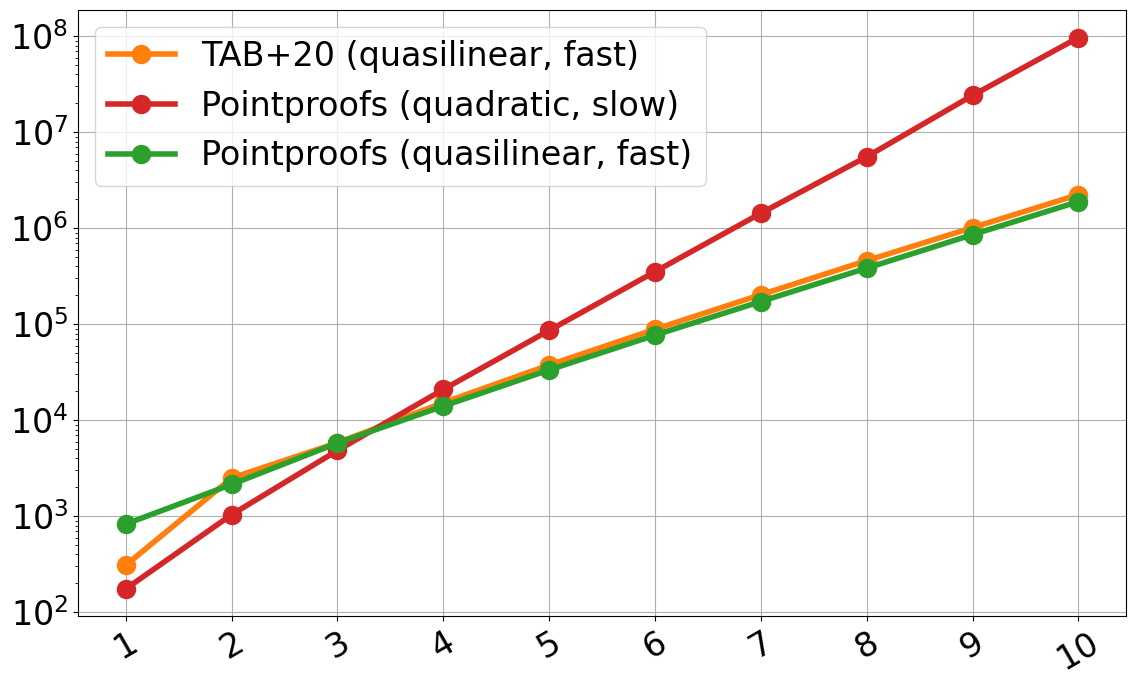
\includegraphics[width=0.50\columnwidth]{fk-vs-pointproofs.png}
    \caption{
        The $x$-axis is $\log_2{N}$, where $N$ is the size of the vector of messages $\vect{m}$.
        The $y$-axis is the time to compute all $N$ proofs for the specified scheme, in microseconds.
    }
    \label{f:benchmarks}
\end{figure}

\section{Conclusion}
In this short paper, we reduced the time to compute all $N$ proofs in the Pointproofs vector commitment scheme from $O(N^2)$ to $O(N\log{N})$.
The key ingredient was representing the proof computation as a product between a Toeplitz matrix and a vector, which can be computed fast via Discrete Fourier Transforms (DFTs) on group elements.
Our implementation shows our $O(N\log{N})$ algorithm is considerably faster when compared to the naive $O(N^2)$ proof precomputation algorithm in Pointproofs.
It is also slightly faster than the FK-based~\cite{FK20} proof precomputation in KZG-based VCs such as~\cite{TAB+20}.

\parhead{Acknowledgements.}
We thank Leonid Reyzin for suggesting to look at Pointproofs from the lens of polynomial commitments, which inspired the author to devise this technique for computing all proofs fast.

\ifEurocrypt
    \bibliographystyle{abbrv}
    %\bibliographystyle{plain}
    {\footnotesize
    \bibliography{references}}
\else
    \clearpage
    \bibliographystyle{alpha}
    \bibliography{references}
\fi


\ifNotEurocrypt
    %\clearpage
\fi

\end{document}
